\documentclass{article}
\usepackage{amsmath}
\usepackage[margin=1in]{geometry}
\usepackage{amsfonts}
\usepackage{hyperref}
\usepackage{graphicx}

\begin{document}
	
\title{Linear Combination}
\author{Andy Chong Sam}

\maketitle	

\section{Visual Intution}
\begin{minipage}[c]{.5\linewidth}
	\par \noindent We first start with the idea of a generic vector which can be scaled by a positive or negative k. As seen on Figure 1, given positive enough or negative values of k, the vector can occupy a line of space.
\end{minipage}%%%
\begin{minipage}[c]{.5\linewidth}
\begin{center}
	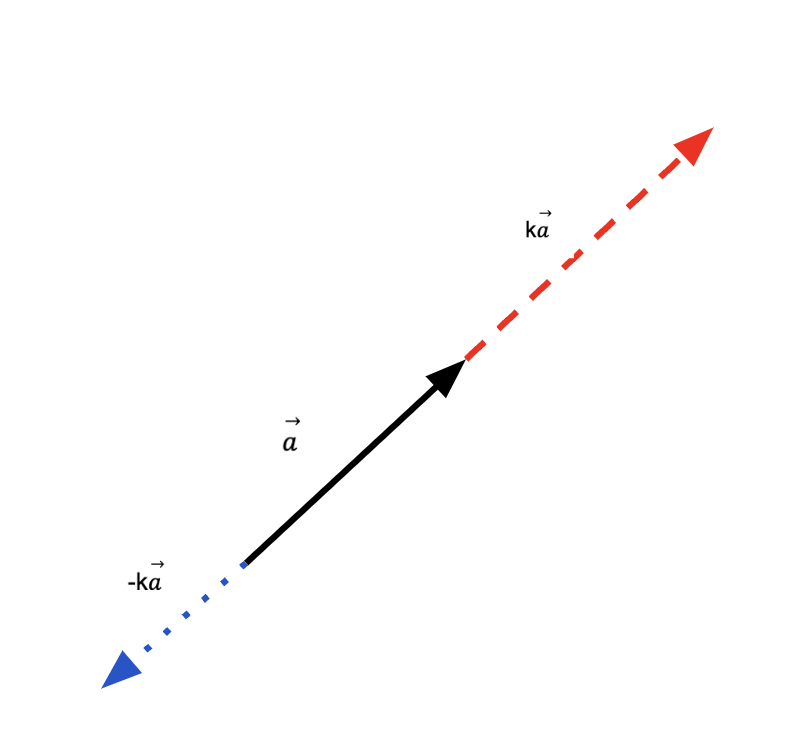
\includegraphics[width=3cm]{matrix-scaling-1.png}
\end{center}
\begin{center}
	Figure 1	
\end{center}
\end{minipage}
\linebreak
\linebreak
\linebreak
\begin{minipage}[c]{.5\linewidth}
	\par \noindent Now suppose we have two vectors \( \vec a \) and \( \vec b \).  They can each be scaled independently. Both vectors can also be added together. With some visual imagination we how by varying the scaling factor of each vector we can reach every point on the two dimensional plane.
\end{minipage}%%%
\begin{minipage}[c]{.5\linewidth}
\begin{center}
	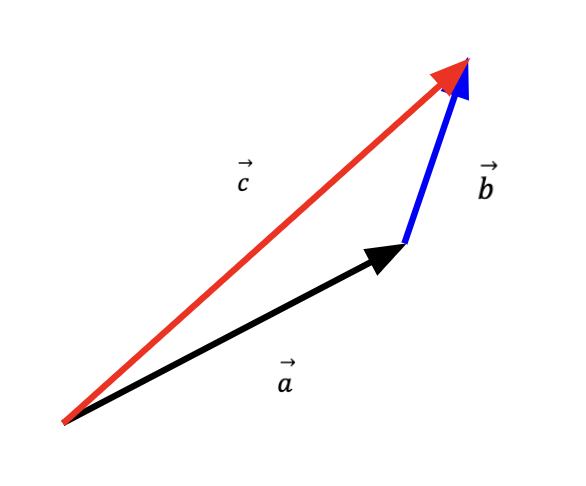
\includegraphics[width=3cm]{vector-scaling-2.png}
\end{center}
\begin{center}
	Figure 2	
\end{center}
\end{minipage}
\linebreak
\linebreak
\linebreak
\begin{minipage}[c]{.5\linewidth}
	\par \noindent We can of course add multiple vectors together, each with the ability to scale independently. A hypothetical situation with three vectors is shown on Figure 3.
\end{minipage}%%%
\begin{minipage}[c]{.5\linewidth}
\begin{center}
	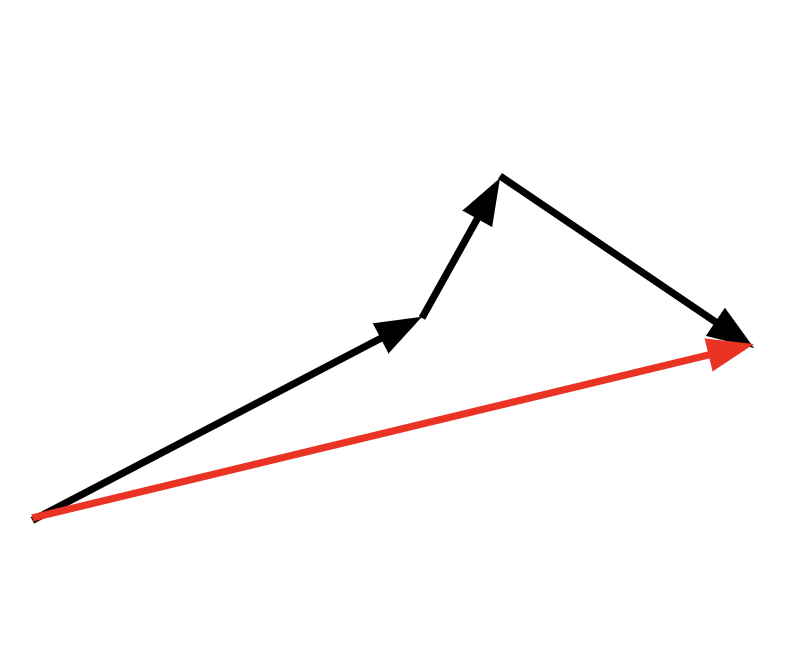
\includegraphics[width=3cm]{matrix-scaling-3.png}
\end{center}
\begin{center}
	Figure 3
\end{center}
\end{minipage}
\newline
\newline
\newline
\par \noindent We can describe describe the summation of n vectors \(<x_n, y_n>\) together like so:
\[
k_1
\left(\begin{array}{@{}c@{}}
	x_1 \\
	y_1 \\
\end{array}\right) + 
k_2
\left(\begin{array}{@{}c@{}}
	x_2 \\
	y_2 \\
\end{array}\right) + 
k_3
\left(\begin{array}{@{}c@{}}
	x_3 \\
	y_3 \\
\end{array}\right) + 
... 
k_n
\left(\begin{array}{@{}c@{}}
	x_n \\
	y_n \\
\end{array}\right) =
\left(\begin{array}{@{}c@{}}
	k_1 x_1 + k_2 x_2 + ... + k_n x_n \\
	k_1 y_1 + k_2 y_2 + ... + k_n y_n \\
\end{array}\right) 
\]
\par \noindent The expression above can be rewritten in the form of a matrix multiplication:
\[
\left(\begin{array}{@{}cccc@{}}
	x_1 & x_2 & ... &x_n\\
	y_1 & y_2 & ... &y_n\\
	
\end{array}\right) 
\left(\begin{array}{@{}c@{}}
	k_1 \\
	k_2 \\
	... \\
	k_n
\end{array}\right) 
\]
\par \noindent It is for this reason that when vectors are written into a matrix they are often done so vertically down a column.


\end{document}